% A before/after presentation demonstration using independent teaching content.
\documentclass[aspectratio=169,11pt]{beamer}
\usepackage{amsmath,amssymb,booktabs,pgfplots}
\pgfplotsset{compat=1.18}
\definecolor{talkblue}{HTML}{185B91}
\definecolor{talkorange}{HTML}{A84D13}
\setbeamercolor{structure}{fg=talkblue}
\setbeamercolor{normal text}{fg=black,bg=white}
\setbeamercolor{frametitle}{fg=talkblue,bg=white}
\setbeamertemplate{navigation symbols}{}
\setbeamertemplate{footline}{\hspace{4mm}\scriptsize Presentation revision examples\hfill\hyperlink{route}{Index}\hspace{1em}\insertframenumber/\inserttotalframenumber\hspace{4mm}\vspace{2mm}}
\setbeamersize{text margin left=8mm,text margin right=8mm}
\setbeamerfont{frametitle}{size=\Large}
\hypersetup{pdftitle={Before and after: mathematical presentation design},pdfauthor={},pdfsubject={Independent examples of slide revision},pdfkeywords={presentation,revision,mathematics}}
\newcommand{\norm}[1]{\left\lVert#1\right\rVert_2}
\newcommand{\editnote}[1]{\par\vfill{\scriptsize\color{talkorange}Design note: #1}}
\newcommand{\errorplot}{%
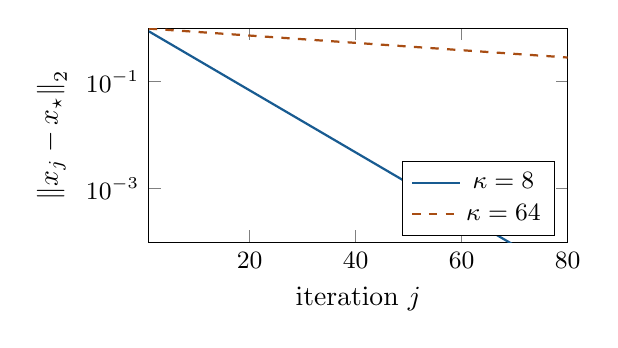
\begin{tikzpicture}
\begin{semilogyaxis}[width=6.9cm,height=4.3cm,xlabel={iteration $j$},ylabel={$\norm{x_j-x_\star}$},xmin=1,xmax=80,ymin=1e-4,ymax=1,legend style={font=\small,at={(.97,.03)},anchor=south east},tick label style={font=\small}]
\addplot[talkblue,thick,domain=1:80,samples=80] {(1-1/8)^x};\addlegendentry{$\kappa=8$}
\addplot[talkorange,dashed,thick,domain=1:80,samples=80] {(1-1/64)^x};\addlegendentry{$\kappa=64$}
\end{semilogyaxis}
\end{tikzpicture}}
\begin{document}

\begin{frame}[label=route]{Before and after: mathematical presentations}
\framesubtitle{The same teaching content, revised for an audience}
\begin{enumerate}
\item \hyperlink{dense-before}{An overloaded page} $\longrightarrow$ \hyperlink{dense-after}{two pages with distinct jobs}
\item \hyperlink{plot-before}{An unexplained result figure} $\longrightarrow$ \hyperlink{plot-after}{an interpretable comparison}
\item \hyperlink{ending-before}{Repeated closing summaries} $\longrightarrow$ \hyperlink{ending-after}{one evidence-based conclusion}
\end{enumerate}
\vspace{4mm}
\small All examples use a standard quadratic problem. No private deck, author identity, or research measurement is reproduced.
\editnote{Blue page headings identify the topic; BEFORE/AFTER labels identify the revision. Orange notes explain editing choices and are not part of a research talk.}
\end{frame}

\begin{frame}[label=dense-before]{1 / BEFORE: one page doing too many jobs}
\framesubtitle{Original specimen: definition, algorithm, theorem, proof, interpretation}
\small
For $x\in\mathbb R^2$, $\kappa\geq1$, $f_\kappa(x)=\frac12(x_1^2+\kappa x_2^2)$, $A=\operatorname{diag}(1,\kappa)$, $x_\star=0$, $x_0=(1,1)^T$, $\eta=1/\kappa$:
\[
\nabla f_\kappa=Ax,\quad x_{j+1}=(I-\eta A)x_j,\quad
x_{1,j+1}=(1-\kappa^{-1})x_{1,j},\quad x_{2,j+1}=0.
\]
In general, for symmetric positive definite $A$ with eigenvalues in $[m,L]$ and $0<\eta<2/L$, $\norm{x_j}\leq q^j\norm{x_0}$ where $q=\max_i|1-\eta\lambda_i|<1$.
\[
A=Q\Lambda Q^T,\quad Q^TQ=I,\quad
Q^Tx_{j+1}=(I-\eta\Lambda)Q^Tx_j.
\]
Orthogonal diagonalization gives independent scalar contractions; in our example $q=1-1/\kappa$. Larger $\kappa$ slows the first coordinate. For $j\geq1$, $\norm{x_j}=(1-1/\kappa)^j$.
\editnote{The mathematics is consistent, but the audience must learn the example and the general theorem at the same time. Smaller text is not the solution.}
\end{frame}

\begin{frame}[label=dense-after]{1 / AFTER A: define the example and expose the obstacle}
\framesubtitle{Job of this page: understand why one direction is slow}
\begin{columns}[T]
\begin{column}{.51\textwidth}
\[
f_\kappa(x)=\tfrac12(x_1^2+\kappa x_2^2),\quad\kappa\geq1.
\]
Minimizer $x_\star=0$; start $x_0=(1,1)^T$.
\[
x_{j+1}=x_j-\kappa^{-1}\nabla f_\kappa(x_j).
\]
\[
x_{1,j+1}=(1-\kappa^{-1})x_{1,j},\qquad x_{2,j+1}=0.
\]
\end{column}
\begin{column}{.43\textwidth}
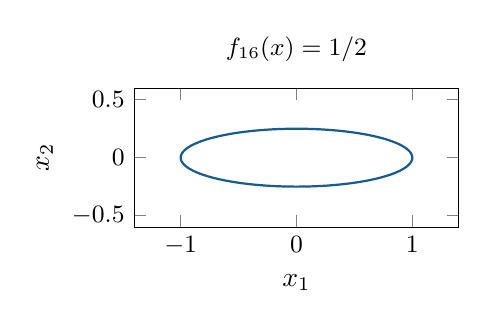
\begin{tikzpicture}
\begin{axis}[width=5.7cm,height=3.8cm,axis equal image,xmin=-1.4,xmax=1.4,ymin=-.6,ymax=.6,xlabel={$x_1$},ylabel={$x_2$},tick label style={font=\small},title={$f_{16}(x)=1/2$},title style={font=\small}]
\addplot[talkblue,thick,domain=0:360,samples=121] ({cos(x)},{sin(x)/4});
\end{axis}
\end{tikzpicture}
\end{column}
\end{columns}
\editnote{Keep the problem and its mechanism together. Move the general theorem to the next page; explain the transition in the speaker notes.}
\end{frame}

\begin{frame}{1 / AFTER B: state the theorem and its decisive step}
\framesubtitle{Job of this page: explain what makes the contraction valid}
Let $A=A^T\succ0$, with $0<m\leq\lambda_i\leq L$.
For $x_{j+1}=(I-\eta A)x_j$ and $0<\eta<2/L$,
\[
\norm{x_j}\leq q^j\norm{x_0},\qquad q=\max_i|1-\eta\lambda_i|<1.
\]
\textbf{Key step:} write $A=Q\Lambda Q^T$, with $Q^TQ=I$.
\[
Q^Tx_{j+1}=(I-\eta\Lambda)Q^Tx_j.
\]
Each component contracts by at most $q$; the norm is unchanged by $Q$.
\smallskip
\small In the preceding example, $q=1-1/\kappa$ and $\norm{x_j}=(1-1/\kappa)^j$ for $j\geq1$.
\editnote{Restore normal text size. Retain the hypotheses and the proof bridge; do not shorten the statement to an unconditional slogan.}
\end{frame}

\begin{frame}[label=plot-before]{2 / BEFORE: a figure without the experiment}
\framesubtitle{Original specimen: ``Convergence results''}
\centering
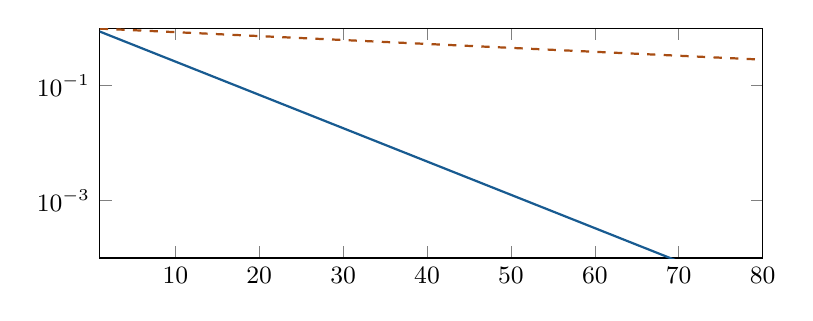
\begin{tikzpicture}
\begin{semilogyaxis}[width=10cm,height=4.5cm,xmin=1,xmax=80,ymin=1e-4,ymax=1,tick label style={font=\small}]
\addplot[talkblue,thick,domain=1:80,samples=80] {(1-1/8)^x};
\addplot[talkorange,dashed,thick,domain=1:80,samples=80] {(1-1/64)^x};
\end{semilogyaxis}
\end{tikzpicture}
\editnote{These curves are real formula evaluations, but their axes, parameters, and purpose are missing. A larger plot does not supply the missing meaning.}
\end{frame}

\begin{frame}[label=plot-after]{2 / AFTER: make the comparison interpretable}
\framesubtitle{What changes: $\kappa$; what is measured: Euclidean error by iteration}
\begin{columns}[T]
\begin{column}{.53\textwidth}
\errorplot
\end{column}
\begin{column}{.43\textwidth}
\small
\textbf{Common problem}
\[
f_\kappa(x)=\tfrac12(x_1^2+\kappa x_2^2).
\]
$x_0=(1,1)^T$, $x_\star=0$; gradient step $\eta=1/\kappa$.
\medskip

\textbf{Exact reference}
\[
\norm{x_j}=(1-1/\kappa)^j,\quad j\geq1.
\]
Larger $\kappa$ gives slower contraction under this step-size rule.
\medskip

This is not a wall-clock comparison.
\end{column}
\end{columns}
\editnote{Keep the same curves. Add only the setup and labels needed to interpret them; use a line style as well as color.}
\end{frame}

\begin{frame}[label=ending-before]{3 / BEFORE: three closing pages repeat the same point}
\framesubtitle{A storyboard of a repetitive ending; each box represents a page}
\begin{columns}[T]
\begin{column}{.31\textwidth}
\begin{block}{Page A: Summary}
Conditioning matters.\par\medskip
The spectrum controls the iteration.
\end{block}
\end{column}
\begin{column}{.31\textwidth}
\begin{block}{Page B: Discussion}
Large $\kappa$ gives slow progress.\par\medskip
Directions behave differently.
\end{block}
\end{column}
\begin{column}{.31\textwidth}
\begin{block}{Page C: Conclusion}
The convergence rate depends on the eigenvalues.\par\medskip
Conditioning is important.
\end{block}
\end{column}
\end{columns}
\editnote{The statements are not false. The problem is repetition without another conclusion, useful limitation, or open question.}
\end{frame}

\begin{frame}[label=ending-after]{3 / AFTER: one closing page tied to the evidence}
\framesubtitle{Replace three repetitive summaries with distinct supported statements}
\small
\begin{tabular}{@{}p{.46\textwidth}p{.46\textwidth}@{}}
\toprule
Conclusion & Support already shown \\
\midrule
The step size must respect the spectrum. & $0<\eta<2/L$ ensures $\max_i|1-\eta\lambda_i|<1$. \\[2mm]
The selected step slows as $\kappa$ grows. & In the example, $q=1-1/\kappa$; the exact curves show this dependence. \\[2mm]
No timing advantage has been established. & The comparison evaluates a recurrence, not solver wall-clock time. \\
\bottomrule
\end{tabular}\par
\vspace{4mm}
\normalsize\raggedright Next question: what changes for a nonquadratic objective, where the curvature varies along the iteration?\par
\editnote{Give the ending a new job: connect claims to evidence and state the next unresolved issue. Keep expanded discussion in the notes.}
\end{frame}

\begin{frame}{A reusable revision procedure}
\begin{enumerate}
\item Identify the page's job and the audience's prerequisites.
\item Keep formulas and assumptions that carry that job.
\item Split, merge, or reorder to repair the dependency chain.
\item Add a figure only if it reveals a mechanism or comparison.
\item Check the revised pages, their transitions, and speaking time.
\end{enumerate}
\vspace{3mm}
\small These are editing decisions, not mandatory page templates. A split is useful only if each resulting page has a distinct role; more slides alone do not make a better talk.
\editnote{Use the companion guide for the edits, rationale, notes, and review criteria. This final page belongs to the demonstration, not the toy research talk.}
\end{frame}
\end{document}
